%!TEX program = xelatex
%!TEX TS-program = xelatex
%!TEX encoding = UTF-8 Unicode

\documentclass{ctexart}
\usepackage{amsmath} 
\usepackage{amssymb} 
\usepackage{graphicx}
\usepackage{hyperref}
\usepackage{enumitem}

\title{LaTeX入门}
\author{Wenh\_q}

\begin{document}
    \maketitle
    
    \section{完成HelloWorld}
一个最小 LaTeX 文档需要以下结构:\\
$\backslash$documentclass\{article\}\\
$\backslash$begin\{document\}\\
hello, world\\
$\backslash$end\{document\}\\

需要标题、作者与注释的文档结构:\\
$\backslash$documentclass\{article\}\\
$\backslash$author\{My Name\}\\
$\backslash$title\{The Title\}\\
$\backslash$begin\{document\}\\
$\backslash$maketitle\\
hello, world \% This is comment\\
$\backslash$end\{document\}\\

    \section{输入中文}
将 $\backslash$documentclass\{article\} 改为 $\backslash$documentclass\{ctexart\}。生成文档会提示缺少包,将缺少的包安装通过即可。ctex 宏包需要CCT 系统或者CJK 宏包的支持。主要文件包括ctexart.cls、 ctexrep.cls、ctexbook.cls 和ctex.sty、ctexcap.sty。 ctex 宏包由ctex.org 制作并负责维护。

    \section{章节和段落}
你好中国,中国在东亚。
        \subsection{你好北京}
北京是中国的首堵。
                \subsubsection{你好东城区}
                \paragraph{天安门广场}是北京的中心
                    \subparagraph{毛主席纪念堂}在天安门广场的中心
        \subsection{你好广州}
        \paragraph{中山大学}是广州最好的大学\cite{LaTeX新人教程}

    \section{数学公式}
展示数学公式和特殊符号需要添加amsmath和amssymb两个包。   \\ 
$\backslash$usepackage\{amsmath\} \\
$\backslash$usepackage\{amssymb\} \\

The Newton's second law is F=ma.

The Newton's second law is $F=ma$.

The Newton's second law is
$$F=ma$$

The Newton's second law is
\[F=ma\]

Greek Letters $\eta$ and $\mu$

Fraction $\frac{a}{b}$

Power $a^b$

Subscript $a_b$

Derivate $\frac{\partial y}{\partial t} $

Vector $\vec{n}$

Bold $\mathbf{n}$

To time differential $\dot{F}$

Matrix (lcr here means left, center or right for each column)
\[
\left[
\begin{array}{lcr}
a1 & b22 & c333 \\
d444 & e555555 & f6
\end{array}
\right]
\]

Equations(here \& is the symbol for aligning different rows)
\begin{align}
a+b&=c\\
d&=e+f+g
\end{align}

\[
\left\{
\begin{aligned}
&a+b=c\\
&d=e+f+g
\end{aligned}
\right.
\]

    \section{插入图片}
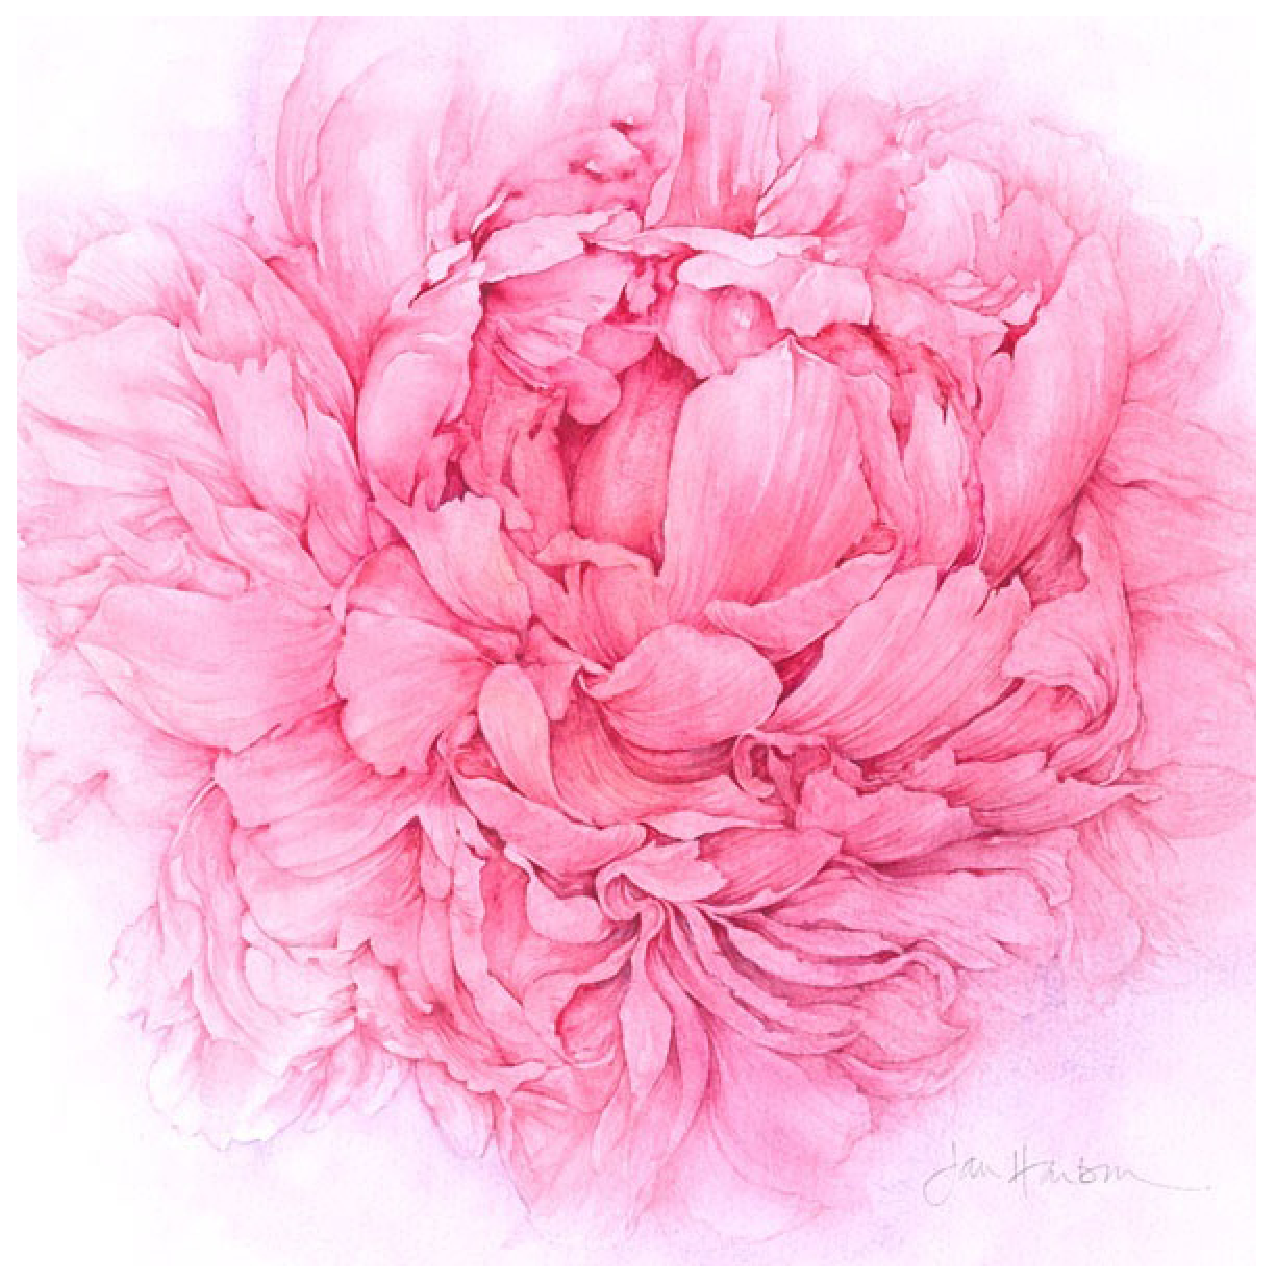
\includegraphics[width=4.00in,height=3.00in]{1.eps}

    \section{表格}
    \paragraph{表格1}
    \begin{tabular}{|c|c|}
    a & b \\
    c &d \\
    \end{tabular}
    
    \paragraph{表格2}
    \begin{tabular}{|c|c|}
    \hline
    a & b \\
    c &d \\
    \hline
    \end{tabular}

    \paragraph{表格3}
    \begin{tabular}{|c|c|}
    \hline
    a & b \\
    \hline
    c &d \\
    \hline
    \end{tabular}

    \paragraph{表格4}
    \begin{center}
    \begin{tabular}{|c|c|}
    \hline
    a & b \\
    \hline
    c &d \\
    \hline
    \end{tabular}
    \end{center}

    \section{宏包}
    \paragraph{} $\backslash$usepackage\{\}就是在调用宏包,每一个宏包里都定义了一些专门的命令,通过这些命令可以实现对于一类对象(如数学公式等)的统一排版(如字号字形),或用来实现一些功能(如插入图片或制作复杂表格)。
    \paragraph{} 常用的宏包有
    \begin{center}
    \begin{tabular}{|c|c|}
    \hline
    编辑数学公式& amsmath和 amssymb \\
    \hline
    编辑数学定理和证明过程 & amsthm \\
    \hline
    插入图片 & graphicx \\
    \hline
    复杂表格 & multirow \\
    \hline
    在文章中使用 $\backslash$url 命令\cite{引用网络资源} & hyperref \\
    \hline
    排序 & enumitem \\
    \hline
    \end{tabular}
    \end{center}

     \paragraph{} 补充说明,现在ctexart模板里集成了中文支持,所以CJK宏包并不是必需品。
    

    \section{BIBTeX制作参考文献}
    \paragraph{} 
    \begin{enumerate}
 \item 用LaTeX编译你的 .tex 文件 , 这是生成一个 .aux 的文件, 这告诉 BibTeX 将使用那些应用。
 \item 用BibTeX 编译 .bib 文件。
 \item 再次用LaTeX 编译你的 .tex 文件, 这个时候在文档中已经包含了参考文献, 但此时引用的编号可能不正确。
 \item 最后用 LaTeX 编译你的 .tex 文件, 如果一切顺利的话, 这是所有东西都已正常了。\cite{Latex中如何制作参考文献}
    \end{enumerate}
    
    \bibliographystyle{plain}
    \bibliography{helloworld.bib}
\end{document}